
\chapter{CPU Description}
\label{cpu_description}

    This section is about the 'core' cpu (mips\_cpu.vhdl), excluding the cache.

    \begin{figure}[h]
    \makebox[\textwidth]{\framebox[9cm]{\rule{0pt}{9cm}
    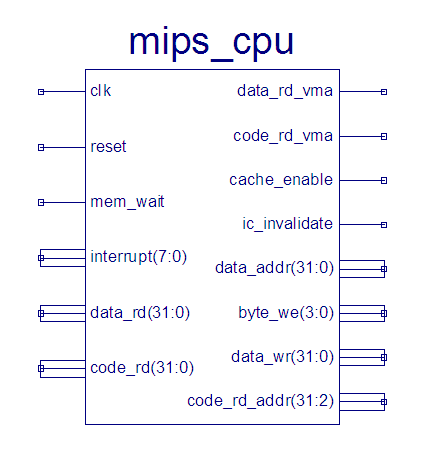
\includegraphics[width=8cm]{img/cpu_symbol.png}}}
    \caption{CPU module interface\label{cpu_symbol}}
    \end{figure}
    
    the CPU module is not meant to be used directly. Instead, the MCU module
    described in section ~\ref{mcu_module} should be used.\\
    
    The following sections will describe the CPU structure and interfaces.\\
    
\section{Bus Architecture}
\label{bus_architecture}
    The CPU uses a Harvard architecture: separate paths for code and data. It
    has three separate, independent buses: code read, data read and data write.
    (Data read and write share the same address bus).\\

    The CPU will perform opcode fetches at the same time it does data reads
    or writes. This is not only faster than a Von Neumann architecture where
    all memory cycles have to be bottlenecked through a single bus; it is much
    simpler too. And most importantly, it matches the way the CPU will work
    when connected to code and data caches.\\

    (Actually, in the current state of the core, due to the inefficient way in
    which load interlocking has been implemented, the core is less efficient
    than that -- more on this later).\\

    The core can't read and write data at the same time; this is a fundamental 
    limitation of the core structure: doing both at the same time would take 
    one more read port in the register bank -- too expensive. Besides, it's not
    necessary given the 3-stage pipeline structure we use.\\

    In the most basic use scenario (no external memory and no caches), code and
    data buses have a common address space but different storages and the
    architecture is strictly Harvard. When cache memory is connected
    the architecture becomes a Modified Harvard -- because data and 
    code ultimately come from the same storage, on the same external 
    bus(es).\\

    Note that the basic cpu module (mips\_cpu) is meant to be connected to 
    internal, synchronous BRAMs only (i.e. the cache BRAMs). Some of its 
    outputs are not registered because they needn't be. The parent module 
    (called 'mips\_mcu') has its outputs registered to limit $t_{co}$ to 
    acceptable values.\\


\subsection{Code and data read bus interface}
\label{code_data_buses}
    Both buses have the same interface:\\
    
\begin{tabular}{ l l }
    $\star$\_rd\_addr  & Address bus\\ 
    $\star$\_rd        & Data/opcode bus\\ 
    $\star$\_rd\_vma   & Valid Memory Address (VMA)\\ 
\end{tabular}\\

    The CPU assumes SYNCHRONOUS external memory (most or all FPGA architectures
    have only synchronous RAM blocks):

    When $\star$\_rd\_vma is active ('1'), $\star$\_rd\_addr is a valid read address and the
    memory should provide read data at the next clock cycle.

    The following ascii-art waveforms depict simple data and code read cycles
    where there is no interlock -- interlock is discussed in section 2.3.\\
    
\needspace{26\baselineskip}
\begin{verbatim}
    ==== Chronogram 3.1.A: data read cycle, no stall ======================
                         ____      ____      ____      ____      ____
     clk            ____/    \____/    \____/    \____/    \____/    \____/

                         _________           _________
     data_rd_vma    ____/         \_________/         \____________________

     data_rd_addr   XXXX| 0x0700  |XXXXXXXXX| 0x0800  |XXXXXXXXX|XXXXXXXXX|

     data_rd        XXXX|XXXXXXXXX| [0x700] |XXXXXXXXX| [0x800] |XXXXXXXXX|

     (target reg)   ????|?????????|?????????| [0x700] |?????????| [0x800] |

              (data is registered here...)--^    (...and here)--^

     ==== Chronogram 3.1.B: code read cycle, no stall =====================
                         ____      ____      ____      ____      ____
     clk            ____/    \____/    \____/    \____/    \____/    \____/

                         __________________________________________________
    code_rd_vma     ____/         |         |         |         |         |

                    ????| 0x0100  | 0x0104  | 0x0108  | 0x010c  | 0x0200  |

    code_rd         XXXX|XXXXXXXXX| [0x100] | [0x104] | [0x108] | [0x10c] |

    p1_ir_reg       ????|?????????|?????????| [0x100] | [0x104] | [0x108] |

      (first code word is registered here)--^

    ========================================================================
\end{verbatim}\\

    The data address bus is 32-bit wide; the lowest 2 bits are redundant in 
    read cycles since the CPU always reads full words, but they may be useful 
    for debugging.\\

\subsection{Data write interface}
\label{data_write_bus}

    The write bus does not have a vma output because byte\_we fulfills the same
    role:\\
   
\begin{tabular}{ l l }
    $\star$\_wr\_addr   & Address bus\\
    $\star$\_wr         & Data/opcode bus\\
    byte\_we            & WE for each of the four bytes
\end{tabular}\\

    Write cycles are synchronous too. The four bytes in the word should be
    handled separately -- the CPU will assert a combination of byte\_we bits
    according to the size and alignment of the store.\\

    When byte\_we(i) is active, the matching byte at data\_wr should be stored
    at address data\_wr\_addr. byte\_we(0) is for the LSB, byte\_we(3) for the MSB.
    Note that since the CPU is big endian, the MSB has the lowest address and
    LSB the highest. The memory system does not need to care about that.\\

    Write cycles never cause data-hazard stalls. They would take a single
    clock cycle except for the inefficient cache implementation, which
    stalls the CPU until the writethrough is done.\\

    This is the waveform for a basic write cycle (remember, this is without
    cache; the cache would just stretch this diagram by a few cycles):

\needspace{20\baselineskip}
\begin{verbatim}

    ==== Chronogram 3.2: data write cycle =================================
                         ____      ____      ____      ____      ____
     clk            ____/    \____/    \____/    \____/    \____/    \____/

     byte_we        XXXX|  1111   |  0000   |  0100   |  1100   |  0000   |

     data_wr_addr   XXXX| 0x0700  |XXXXXXXXX| 0x0800  | 0x0900  |XXXXXXXXX|

     data_wr        XXXX|12345678h|XXXXXXXXX|12345678h|12345678h|XXXXXXXXX|

     [0x0700]       ????|????????h|12345678h|12345678h|12345678h|12345678h|

     [0x0800]       ????|????????h|????????h|????????h|??34????h|??34????h|

     [0x0900]       ????|????????h|????????h|????????h|????????h|1234????h|

    ========================================================================
\end{verbatim}\\

    Note the two back-to-back stores to addresses 0x0800 and 0x0900. They are
    produced by two consecutive S$\star$ instructions (SB and SH in the example),
    and can only be done this fast because of the Harvard architecture (and,
    again, because the diagram does not account for the cache interaction).
    
    
\subsection{CPU stalls caused by memory accesses}
\label{memory_cpu_stalls}

    In short, the 'mem\_wait' input will unconditionally stall all pipeline
    stages as long as it is active. It is meant to be used by the cache at cache 
    refills.\\

    In short, the cache/memory controller stops the cpu for all data/code 
    misses for as long as it takes to do a line refill. The current cache 
    implementation does refills in order (i.e. not 'target address first').

    Note that external memory wait states are a separate issue. They too are 
    handled in the cache/memory controller. See section~\ref{cache} on the memory
    controller.

\section{Pipeline}
\label{pipeline}

    Here is where I would explain the structure of the cpu in detail; these 
    brief comments will have to suffice until I write some real documentation.\\
    
    This section could really use a diagram; since it can take me days to draw 
    one, that will have to wait for a further revision.\\
    
    This core has a 3-stage pipeline quite different from the original 
    architecture spec. Instead of trying to use the original names for the
    stages, I'll define my own.\\
    
    A computational instruction of the I- or R- type goes through the following
    stages during execution:\\

    \begin{tabular}{ l l }
        FETCH-0   & Instruction address is in code\_rd\_addr bus\\
        FETCH-1   & Instruction opcode is in code\_rd bus\\
        ALU/MEM   & ALU operation or memory read/write cycle is done OR\\
                  &   Memory read/data address is on data\_rd/wr\_address bus OR\\
                  &   Memory write data is on data\_wr bus\\
        LOAD      & Memory read data is on data\_rd bus
    \end{tabular}\\        
    
    In the core source (mips\_cpu.vhdl) the stages have been numbered:\\
    
    \begin{tabular}{ l l }
        FETCH-1 & = stage 0\\
        ALU/MEM & = stage 1\\
        LOAD    & = stage 2
    \end{tabular}\\  
    
    Here's a few examples:\\

\needspace{9\baselineskip}
\begin{verbatim}
    ==== Chronogram 3.3.A: stages for instruction "lui gp,0x1" ============
                         ____      ____      ____      ____      ____
     clk            ____/    \____/    \____/    \____/    \____/    \____/

     code_rd_addr       | 0x099c  |                                        
     
     code_rd_data                 |3c1c0001h|

     rbank[$gp]                             | 0x0001  |
     
                        |< fetch0>|<   0   >|<   1   >|
    =======================================================================
\end{verbatim}\\


\needspace{17\baselineskip}
\begin{verbatim}
    ==== Chronogram 3.3.B: stages for instruction "lw a0,16(v0)" ==========
                         ____      ____      ____      ____      ____
     clk            ____/    \____/    \____/    \____/    \____/    \____/

     code_rd_addr       | 0x099c  |                                        
     
     code_rd_data                 |8c420010h|
     
     data_rd_addr                           | $v0+16  |
                                             _________
     data_rd_vma                       _____/         \______
     
     data_rd                                          | <data>  |

     rbank[$a0]                                                 | <data>  |
     
                        |< fetch1>|<   0   >|<   1   >|<   2   >|
    ========================================================================
\end{verbatim}\\

    In the source code, all registers and signals in stage 
    \textless i\textgreater are prefixed by 
    "p\textless i\textgreater\_", as in p0\_*, p1\_* and p2\_*. 
    A stage includes a set of registers and 
    all the logic that feeds from those registers (actually, all the logic
    that is between registers p0\_* and p1\_* belongs in stage 0, and so on).
    Since there are signals that feed from more than one pipeline stage (for
    example p2\_wback\_mux\_sel, which controls the register bank write port 
    data multiplexor and feeds from p1 and p2), the naming convention has to be
    a little flexible.\\
    
    FETCH-0 would only include the logic between p0\_pc\_reg and the code ram 
    address port, so it has been omitted from the naming convention.\\
    
    All read and write ports of the register bank are synchronous. The read 
    ports belong logically to stage 1 and the write port to stage 2.\\
    
    IMPORTANT: though the register bank read port is synchronous, its data can
    be used in stage 1 because it is read early (the read port is loaded at the 
    same time as the instruction opcode). That is, a small part of the 
    instruction decoding is done on stage FETCH-1. Bearing in mind that the code 
    ram is meant to be the exact same type of block as the register bank (or 
    faster if the register bank is implemented with distributed RAM), and we 
    will cram the whole ALU delay plus the reg bank delay in stage 1, it does 
    not hurt moving a tiny part of the decoding to the previous cycle.\\
    
    All registers but a few exceptions belong squarely to one of the pipeline
    stages:\\
    
    \begin{tabular}{ l l }
    Stage 0:                                & \\
    p0\_pc\_reg                             & PC \\
    (external code ram read port register)  & Loads the same as PC \\
                                            & \\
    Stage 1:                                & \\
    p1\_ir\_reg                             & Instruction register \\
    (register bank read port register)      &  \\
    p1\_rbank\_forward                      & Feed-forward data (hazards) \\
    p1\_rbank\_rs\_hazard                   & Rs hazard detected \\
    p1\_rbank\_rt\_hazard                   & Rt hazard detected \\
                                            & \\
    Stage 2:                                & \\
    p2\_exception                           & Exception control \\
    p2\_do\_load                            & Load from data\_rd \\
    p2\_ld\_*                               & Load control\\
    (register bank write port register)     & \\
    \end{tabular}\\  
    
    Note how the register bank ports belong in different stages even if it's
    the same physical device. No conflict here, hazards are handled properly
    (logic defined with explicit vendor-independent vhdl code, not with 
    synthesis pragmas, etc.).\\

    There is a small number of global registers that don't belong to any 
    pipeline stage:\\
    
    \begin{tabular}{ p{4cm} l }
    pipeline\_stalled                        & Together, these two signals...\\
    pipeline\_interlocked                    & ...control pipeline stalls
    \end{tabular}\\
    
    
    And of course there are special registers accessible to the CPU programmer 
    model:\\
    
    \begin{tabular}{ p{4cm} l }
        mdiv\_hi\_reg     & register HI from multiplier block\\
        mdiv\_lo\_reg     & register LO from multiplier block\\
        cp0\_status      & register CP0[status]\\
        cp0\_epc         & register CP0[epc]\\
        cp0\_cause       & register CP0[cause]
    \end{tabular}\\
    
    These belong logically to pipeline stage 1 (can be considered an extension
    of the register bank) but have been spared the prefix for clarity.\\

    Note that the CP0 status and cause registers are only partially implemented.\\

    Again, this needs a better explaination and a diagram.\\


\section{Interlocking and Data Hazards}
\label{interlocking_and_data_hazards}

    There are two data hazards we need to care about:\\
    
    a) If an instruction needs to access a register which was modified by the
    previous instruction, we have a data hazard -- because the register bank is
    synchronous, a memory location can't be read in the same cycle it is updated
    -- we will get the pre-update value.
    
    b) A memory load into a register Rd produces its result a cycle late, so if
    the instruction after the load needs to access Rd there is a conflict.\\


    Conflict (a) is solved with some data forwarding logic: if we detect the
    data hazard, the register bank uses a 'feed-forward' value instead of the
    value read from the memory file. \\
    In file mips\_cpu.vhdl, see process 'data\_forward\_register' and the following
    few lines, where the hazard detection logic and data register and 
    multiplexors are implemented. Note that hazard is detected separately for
    both read ports of the reg bank (p0\_rbank\_rs\_hazard and p0\_rbank\_rt\_hazard).
    Note too that this logic is strictly regular vhdl code -- no need to rely here
    on the synthesis tool to add the bypass logic for us. This gets us some
    measure of vendor independence.\\
    
    As for conflict (b), in the original MIPS-I architecture it was the job
    of the programmer to make sure that a loaded value was not used before it
    was available -- by inserting NOPs after the load instruction, if necessary.
    This is what I call the 'load delay slot', as discussed in \cite[p.~13-1]{r3k_ref_man}.\\
    
    The C toolchain needs to be set up for MIPS-I compliance in order to build
    object code compatible with this scheme.\\
    But all succeeding versions of the MIPS architecture implement a 
    different scheme instead, 'load interlock' (\cite[p.~28]{see_mips_run}). You often see
    this behavior in code generated by gcc, even when using the -mips1 flag (this 
    is probably due to the precompiled support code or libc, I have to check).\\
    In short, it pays to implement load interlocks so this core does, but the
    feature should be optional through a generic.\\
    
    
    Load interlock is triggered in stage 1 (ALU/MEM) of the load instruction;
    when triggered, the pipeline stages 0 and 1 stall, but the pipeline stage
    2 is allowed to proceed. That is, PC and IR are frozen but the value loaded
    from memory is written in the register bank.\\
    
    In the current implementation, the instruction following the load is 
    UNCONDITIONALLY stalled; even if it does not use the target register of the 
    load. This prevents, for example, interleaving read and write memory cycles
    back to back, which the CPU otherwise could do.\\
    So the interlock should only be triggered when necessary; this has to be
    fixed.\\

    
\needspace{17\baselineskip}
\begin{verbatim}
    ==== Chronogram 3.4.A: data read cycle, showing interlock =============
                         ____      ____      ____      ____      ____
     clk            ____/    \____/    \____/    \____/    \____/    \____/

     code_rd_addr   XXXX| 0x099c  | 0x09a0            | 0x09a4  | 0x09a8  |
     
     byte_we        XXXX|  0000   |  1111   |  0000   |  0000   |  1100   |
     
                                            |<                 >|
                    ________________________           ____________________
     code_rd_vma                            \_________/               
                                             _________                    
     data_rd_vma    ________________________/         \____________________

     data_rd_addr   XXXX|XXXXXXXXX|XXXXXXXXX| 0x0700            |XXXXXXXXX|

     data_rd        XXXX|XXXXXXXXX|XXXXXXXXX|XXXXXXXXX| [0x700] |XXXXXXXXX|

     (target reg)   ????|?????????|?????????|?????????| [0x700] |?????????|

                           (data is registered here)--^

    ========================================================================
\end{verbatim}\\

    Note how a fetch cycle is delayed.

    This waveform was produced by this code:

\begin{verbatim}    
                ...
                998:    ac430010    sw  v1,16(v0)
                99c:    80440010    lb  a0,16(v0)
                9a0:    a2840000    sb  a0,0(s4)
                9a4:    80440011    lb  a0,17(v0)
                9a8:    00000000    nop
                ...
\end{verbatim}\\

    Note how read and write cycles are spaced instead of being interleaved, as
    they would if interlocking was implemented efficiently (in this example, 
    there was a real hazard, register \$a0, but that's coincidence -- I need to
    find a better example in the listing files...).
    
    
\section{Exceptions}
\label{exceptions}

    The only exceptions supported so far are software exceptions, and of those 
    only the instructions BREAK and SYSCALL, the 'unimplemented opcode' trap and
    the 'user-mode access to CP0' trap.\\
    Memory privileges are not and will not be implemented. Hardware/software 
    interrupts are still unimplemented too.\\
    
    Exceptions are meant to work as in the R3000 CPUs except for the vector 
    address.\\
    They save their own address to EPC, update the SR, abort the following 
    instruction, and jump to the exception vector 0x0180. All as per the specs 
    except the vector address (we only use one).\\
        
    The following instruction is aborted even if it is a load or a jump, and 
    traps work as specified even from a delay slot -- in that case, the address
    saved to EPF is not the victim instruction's but the preceding jump 
    instruction's as explained in \cite[p.~64]{see_mips_run}.\\
    
    Plasma used to save in epc the address of the instruction after break or 
    syscall, and used an unstandard vector address (0x03c). This core will go 
    the standard R3000 way instead.\\
    
    Note that the epc register is not used by any instruction other than mfc0.
    RTE is implemented and works as per R3000 specs.\\


\section{Multiplier}
\label{multiplier}

    The core includes a multiplier/divider module which is a slightly modified 
    version of Plasma's multiplier unit. Changes have been commented in the 
    source code.\\
    
    The main difference is that Plasma does not stall the pipeline while a 
    multiplication/division is going on. It only does when you attempt to get 
    registers HI or LO while the multiplier is still running. Only then will
    the pipeline stall until the operation completes.\\
    This core instead stalls always for all the time it takes to do the 
    operation. Not only it is simpler this way, it will also be easier to 
    abort mult/div instructions.\\
    
    The logic dealing with mul/div stalls is a bit convoluted and coud use some
    explaining and some ascii chronogram. Again, TBD.\\